\def\pathToRoot{../../}\input{\pathToRoot headers/uebungHeader}

\graphicspath{{graphics/}}


\begin{document}
\uebunghead{Talk 12}{Monoidal categories and string diagrams}
\author{Felix Rech}


\begin{exercise}
  Let $A$, $B$, $C$, $D$, be objects in a monoidal category.
  Construct a morphism
  \[
    \roundddd{\rounddd{(A \otimes I) \otimes B} \otimes C} \otimes D
    \to A \otimes \roundddd{B \otimes \rounddd{C \otimes (I \otimes D)}}.
  \]
  Can you find another?
\end{exercise}


\begin{exercise}
  Convert the following algebraic equations into graphical language.
  Which would you expect to be true in any symmetric monoidal category?
  \begin{enumerate}
    \item
      $(g \otimes 1) \of \sigma \of (f \otimes 1)
        = (f \otimes 1) \of \sigma \of (g \otimes 1)$ \\
      for $A \xrightarrow{f, g} A$.

    \item
      $h \of (1 \otimes \lambda) \of (1 \otimes (f \otimes 1)) \of (1 \otimes \lambda^{-1}) \of g
        = h \of g \of \lambda \of (f \otimes 1) \of \lambda^{-1}$ \\
      for $A \xrightarrow{g} B \otimes C$, $I \xrightarrow{f} I$ and $B \otimes C \xrightarrow{h} D$.

    \item
      $\rho \of (1 \otimes f) \of \alpha \of (\sigma \otimes 1)
        = \lambda \of (f \otimes 1) \of \alpha^{-1} \of (1 \otimes \sigma) \of \alpha$ \\
      for $A \otimes B \xrightarrow{f} I$.
  \end{enumerate}
\end{exercise}


\begin{exercise}
    Consider the following diagrams in the graphical calculus:

    \centering 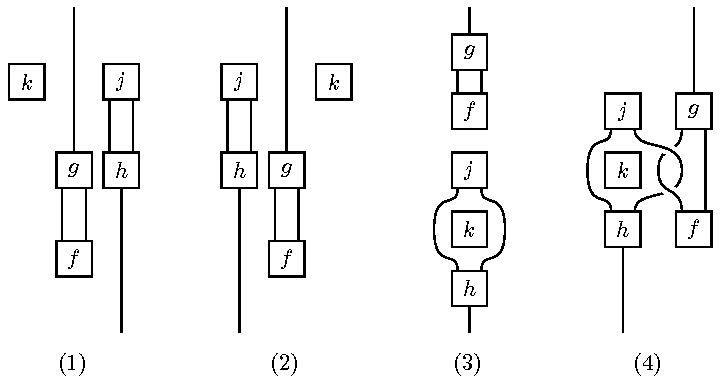
\includegraphics{monoidal-braided-symmetric-comparison}

    \begin{enumerate}
      \item Which diagrams are equal as morphisms in a monoidal category?
      \item Which diagrams are equal as morphisms in a braided monoidal category?
      \item Which diagrams are equal as morphisms in a symmetric monoidal category?
    \end{enumerate}
\end{exercise}


\pagebreak
\begin{exercise}
  Verify the correctness of the following graphical equations in braided monoidal categories by
  \begin{enumerate}
    \item the correctness theorem of the graphical calculus,
    \item substitution in string diagrams using the axioms of braided monoidal categories and the correctness theorem for the graphical calculus on general monoidal categories,
    \item construction of a commuting diagram from the axioms and the coherence theorem for general monoidal categories.
  \end{enumerate}
  \begin{enumerate}[label=(\roman*)]
    \item $\vcenter{\hbox{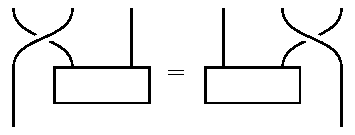
\includegraphics{proofs_by_hand_1}}}$
    \item $\vcenter{\hbox{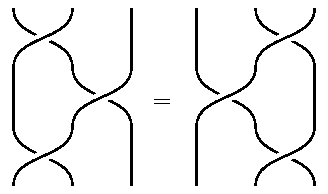
\includegraphics{proofs_by_hand_2}}}$
    \item $\vcenter{\hbox{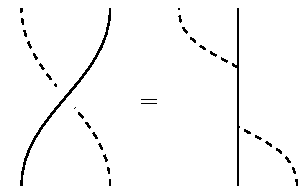
\includegraphics{proofs_by_hand_3}}}$
      ($\sigma_{A, I} = \lambda_{A}^{-1} \of \rho_A$)
  \end{enumerate}
\end{exercise}


\begin{exercise}
  Show that $\Set$ is a symmetric monoidal category under $I \coloneqq \emptyset$ and $A \otimes B \coloneqq A + B + (A \times B)$, where we write $\times$ for Cartesian product of sets and $+$ for disjoint union of sets.
\end{exercise}


\begin{exercise}
  Assume that we have morphisms $I \xrightarrow{\eta} R \otimes L$ and $L \otimes R \xrightarrow{\varepsilon, \varepsilon'} I$ in a monoidal category such that $\eta$ and $\varepsilon$ satisfy one snake equation and $\eta$ and $\varepsilon'$ satisfy the other snake equation.
  Show that this already implies $\varepsilon = \varepsilon'$.
\end{exercise}


\begin{exercise}
  In a monoidal category, show that
  \begin{enumerate}
    \item if an initial object $0$ exists and $L \dashv R$, then $L \otimes 0 \iso 0 \iso 0 \otimes R$;
    \item if a terminal object $1$ exists and $L \dashv R$, then $R \otimes 1 \iso 1 \iso 1 \otimes L$.
  \end{enumerate}
\end{exercise}


\begin{definition}{Idempotent, splitting}
  An endomorphism $A \xrightarrow{f} A$ is called \demph{idempotent} when $f \of f = f$. An idempotent $A \xrightarrow{f} A$ \demph{splits} when there exists an object $B$ and morphisms $A \xrightarrow{g} B$ and $B \xrightarrow{h} A$ such that $f = h \of g$ and $g \of h = 1$.
\end{definition}


\begin{exercise}
  Show that in a monoidal category where all idempotents split, if there are morphisms $I \xrightarrow{\eta} R \otimes L$ and $L \otimes R \xrightarrow{\varepsilon} I$ satisfying one of the snake equations, then $L$ has a right dual (not necessarily given by $R$ with $\eta$ and $\varepsilon$).
\end{exercise}


\end{document}

%%% Local Variables:
%%% mode: latex
%%% TeX-master: t
%%% End:
